\section{Implementation}
\label{sec:impl}

This section describes how the artefact was built (Section~\ref{sec:construction}) and how it was validated (Section~\ref{sec:validation}). It links each step to the problem statement: producing trustworthy, locally actionable skincare guidance.

\subsection{Construction of the Artefact}
\label{sec:construction}

\subsubsection*{Iteration 1: disease and skin-type prototype (August 2026)}

The first version followed the interim plan. Images from several Kaggle collections were merged into folders for seven conditions (including carcinoma) and three skin types. A multi-task EfficientNetB0 was trained on these folders. The Streamlit and mobile interfaces showed the predicted condition, and a carcinoma prediction triggered a ``see a dermatologist'' message.

This iteration proved that the full pipeline could be integrated, from photo to API to recommendations. However, as the progress review recorded, it produced no trustworthy metrics. Manual trials also suggested poor real-world accuracy.

\subsubsection*{Iteration 2: data audit (September 2026)}

Rather than tune the model further, the data was audited. This proved to be the most important decision in the project. Table~\ref{tab:audit} summarises the findings across more than 26,000 files drawn from the original folders and four additional candidate collections.

\begin{table}[ht]
\centering\small
\caption{Findings of the vision data audit}
\label{tab:audit}
\begin{tabular}{lr}
\toprule
\textbf{Finding} & \textbf{Count}\\
\midrule
Files audited & 26,000+\\
Pre-generated (already augmented) images & 2,600+\\
Exact-duplicate groups / images involved & 3,200+ / 7,200+\\
Perceptual-duplicate groups / images involved & 5,200+ / 14,900+\\
Perceptual groups spanning different sources & 2,400+\\
Images passing the strict full-face gate & 3,900+\\
\bottomrule
\end{tabular}
\end{table}

More than half of all images belonged to a perceptual-duplicate group. Thousands of duplicates crossed source boundaries, which shows that the Kaggle collections had re-uploaded each other. The ``cleaned'' train/validation split that came with the original data contained repeated stock images and augmentations, so it leaked into its own validation set. Any accuracy measured on it would have been inflated \citep{barz2020}.

The skin-type folder held only 100+ images, including stock photographs whose labels could not be verified. The condition folders mixed medical diagnoses with cosmetic appearance and had no provenance.

These findings led to three decisions:
\begin{enumerate}
  \item drop disease labels, and with them any implied medical claim;
  \item stop predicting skin type from photographs and ask the user instead;
  \item redefine the task as five visible cosmetic concerns, labelled by a human against written definitions.
\end{enumerate}
The source registry (Table~\ref{tab:sources}) records the outcome for every source.

\begin{table}[ht]
\centering\small
\caption{Source registry decisions}
\label{tab:sources}
\begin{tabularx}{\linewidth}{lllY}
\toprule
\textbf{Source} & \textbf{Images} & \textbf{Decision} & \textbf{Reason}\\
\midrule
Original condition folders & 7,600+ & Partial & Only acne, dark-spot and rosacea folders reviewed; no provenance\\
Kaggle facial skin concerns & 4,200+ & Partial & Useful coverage; watermarks and label noise\\
Kaggle skin issues v2 & 9,700+ & Pending & Unknown licence; heavy overlap\\
Original ``cleaned'' split & 3,200+ & Rejected & Stock images, augmentations, leakage\\
Kaggle normal/oily/dry & 1,400+ & Rejected & Stock images, invalid skin-type labels\\
Original skin-type folder & 100+ & Rejected & Too small; photo-based skin type out of scope\\
ACNE04 \citep{wu2019acne} & 390+ & Accepted & Academic dataset, known provenance\\
FFHQ-Wrinkle \citep{moon2024} & 1,000 & Accepted & Manual wrinkle masks, CC BY-NC-SA\\
SCIN \citep{ward2024} & 70 & Quarantined & 0 of 70 passed the full-face gate; no cosmetic labels\\
PASCAL VOC 2007 \citep{everingham2010} & 300 & Test only & Non-face images for face-gate testing\\
\bottomrule
\end{tabularx}
\end{table}

\subsubsection*{Iteration 3: annotation, training and deployment}

A review queue of 1,400+ images, balanced by source and concern, was labelled in a custom Streamlit annotator. Of these, 1,100+ images were accepted and the rest were rejected as unusable. Most labels remained \emph{unknown}, which is the honest answer for close-ups showing one region.

Negative examples were very scarce. In the first gold set, fewer than 20 images were labelled as having no blemishes, and fewer than 35 as having no redness. Fine lines had the most balanced labels, so FFHQ-Wrinkle was added to strengthen that concern.

The first manifests contained 2,000+ images. Training used seed 42, horizontal-flip, rotation and contrast augmentation, and the two-phase schedule described in Section~\ref{sec:design}. Training refuses to overwrite existing weights, so every run is preserved. This model (\texttt{concern\_v2}) was deployed first, and its weak results for blemishes, redness and pores (Section~\ref{sec:validation}) were traced to the very small number of negative training labels: only 9 for blemishes and 19 each for redness and pores.

Two further engineering problems were found and fixed during this iteration.

\begin{itemize}
  \item \textbf{Train/serve preprocessing mismatch.} The backend originally resized images with a different method from the one used in training. Moving preprocessing into one shared module raised the pooled label accuracy of \texttt{concern\_v2} on the test set from 70.3\% to 73.2\% with no retraining. This shows how silent inconsistencies can erode deployed performance.
  \item \textbf{Degenerate thresholds.} Choosing thresholds by maximising F1 on validation data set the dark-spot and pore thresholds to 0.0, so those concerns were \emph{always} reported as present. Switching to Youden's $J$, which rewards specificity as well as recall, produced meaningful thresholds (Table~\ref{tab:results}).
\end{itemize}

\subsubsection*{Iteration 4: second label review and retraining}

Two attempts were made to fix the shortage of negative examples.
\begin{itemize}
  \item \textbf{Class reweighting} gave each concern's positive and negative labels equal total weight. It did not help on the test set and was rejected (Table~\ref{tab:modelcompare}).
  \item \textbf{A second human review} targeted the 200 training images whose dark-spot, redness or pore labels were still unknown. Every image was re-examined against the same guide. The merge filled 868 previously unknown labels and removed five images judged unusable. Seven disagreements with existing fine-line labels were logged and the original labels were kept. Validation and test files were copied unchanged and verified by hash.
\end{itemize}

The second review raised the number of negative training labels sharply: from 9 to 159 for blemishes, from 19 to 188 for redness, and from 19 to 71 for visible pores (Table~\ref{tab:splits}). The model was then fine-tuned from the \texttt{concern\_v2} weights with the same seed and no class reweighting. The best checkpoint on validation macro ROC-AUC was selected (0.706, compared with 0.686 for \texttt{concern\_v2}). Its thresholds were again chosen on validation data only. This model, \texttt{concern\_human\_reviewed}, scored higher than \texttt{concern\_v2} on all four macro test metrics and is now the deployed model.

A final experiment added 120+ melasma photographs from the MEMI dataset to the training split as extra dark-spot positives. It did not improve dark spots and lowered overall accuracy, so it was not deployed.

\begin{table}[ht]
\centering\small
\caption{Data splits of the deployed model (positive/negative known labels; unknown labels are excluded from the loss)}
\label{tab:splits}
\begin{tabular}{lrrrrrr}
\toprule
\textbf{Split} & \textbf{Images} & \textbf{Blemishes} & \textbf{Dark spots} & \textbf{Redness} & \textbf{Pores} & \textbf{Fine lines}\\
\midrule
Train & 1,200+ & 274/159 & 204/188 & 249/188 & 228/71 & 362/390\\
Validation & 400+ & 68/4 & 36/22 & 64/6 & 33/11 & 123/95\\
Test & 470+ & 97/4 & 65/22 & 97/8 & 46/9 & 116/118\\
\bottomrule
\end{tabular}
\end{table}

\subsubsection*{Catalogue and recommender}

Scraping produced 700+ ForEveryNG, 1,000+ Jeevee and 90+ Oriflame rows. After normalisation and fuzzy deduplication, 1,500+ unique products remained: 800+ from Jeevee, 600+ from ForEveryNG and 70+ from Oriflame. They cover 650+ brands, with a median price of Rs.~799, and 99\% of them are in stock.

Keyword inference assigned a category to 82\% of products. However, it found at least one target ingredient for only 35\% of products (500+), and a skin-type tag for 38\%, because most listings name only headline actives. This limits the ingredient component of the score (Section~\ref{sec:eval}).

\subsubsection*{Mobile application}

The Expo client has four tabs: Chat, Shop, Saved and Settings. Photos are added from the chat screen (the ``+'' button), which keeps analysis and follow-up questions in one conversation. Results open a detail screen with the following elements:
\begin{itemize}
  \item score bars with a threshold tick;
  \item the status of each concern;
  \item a morning and evening routine;
  \item recommendations grouped by category, with ``Fits'' ingredient tags.
\end{itemize}
The server address is discovered automatically on the local network, and structured API errors are translated into plain-language messages. Figure~\ref{fig:screens} shows screenshots captured from the running application.

\textbf{User journey.} A first-time user opens the app on the Chat tab, where an empty-state prompt invites them to tap ``+'' to check a photo or to type a question. Before any analysis, the user can set a skin type in Settings; the screen states that skin type is ``never guessed from photos'', and it may be left unset. Tapping ``+'' offers the camera or the gallery, with an instruction to use ``one clear, front-facing photo of your whole face in daylight''. The result appears as a card that opens the detail screen. Tapping a product opens its detail page, where it can be saved to the user's ``shelf''. Every result is stored in the on-device history under the Saved tab, and the assistant receives the latest result as context, so follow-up questions can refer to the user's own concerns and recommended products.

\begin{figure}[p]
\centering
\begin{subfigure}[t]{0.24\linewidth}
\includegraphics[width=\linewidth]{figures/chat.png}\caption{Grounded chat}\end{subfigure}\hfill
\begin{subfigure}[t]{0.24\linewidth}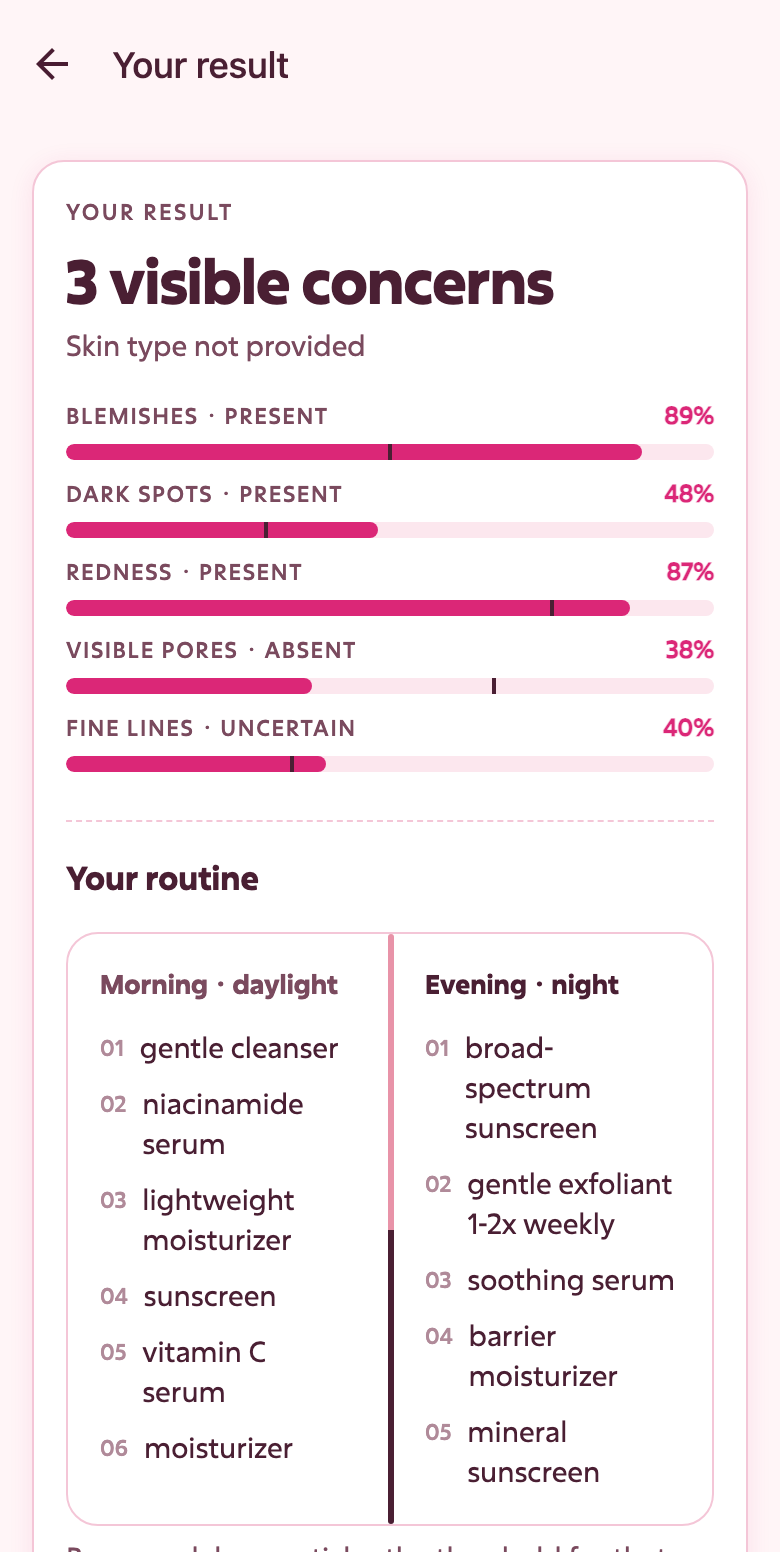
\includegraphics[width=\linewidth]{figures/analysis.png}\caption{Concern result}\end{subfigure}\hfill
\begin{subfigure}[t]{0.24\linewidth}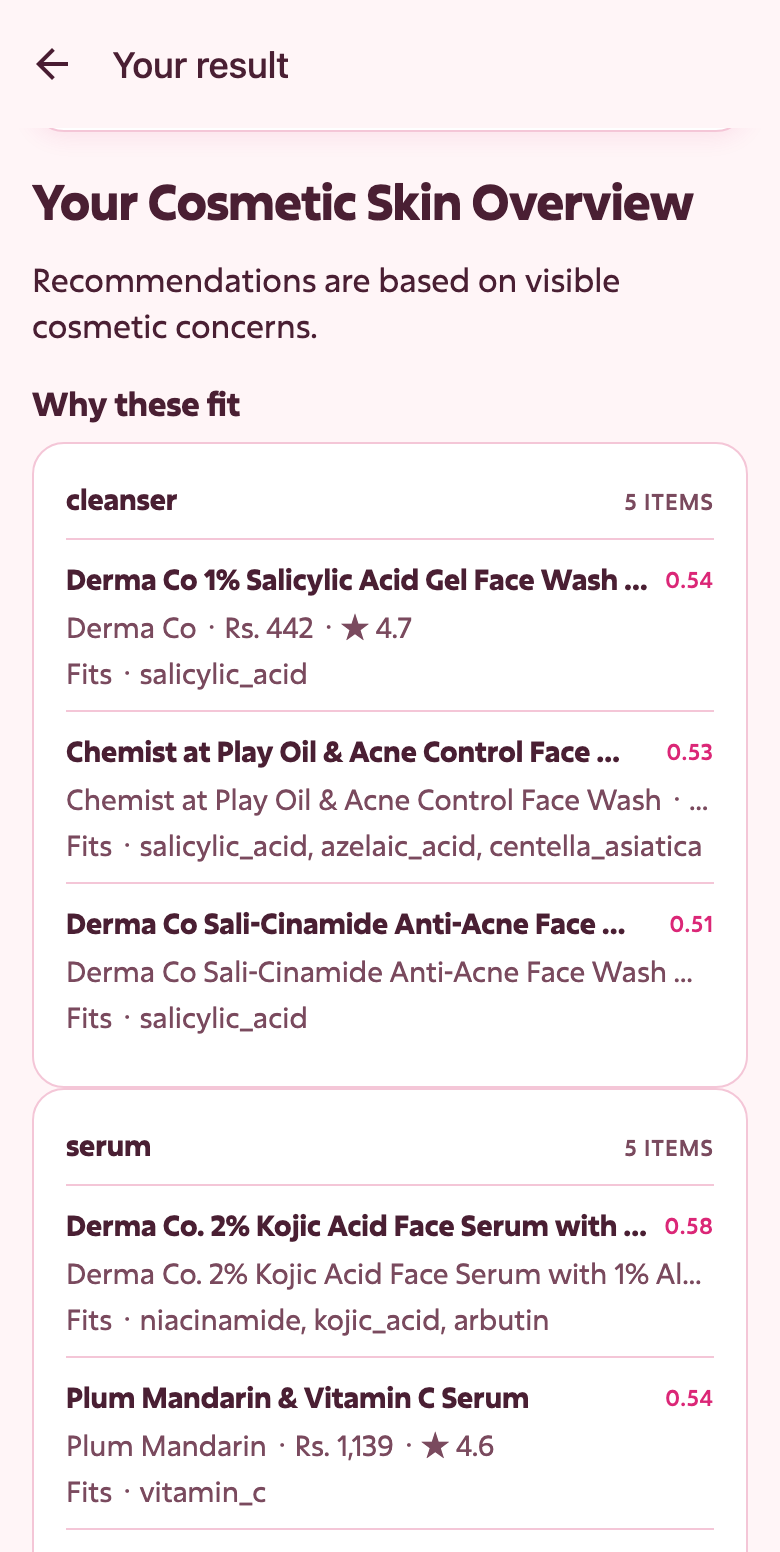
\includegraphics[width=\linewidth]{figures/analysis_1.png}\caption{Recommendations}\end{subfigure}\hfill
\begin{subfigure}[t]{0.24\linewidth}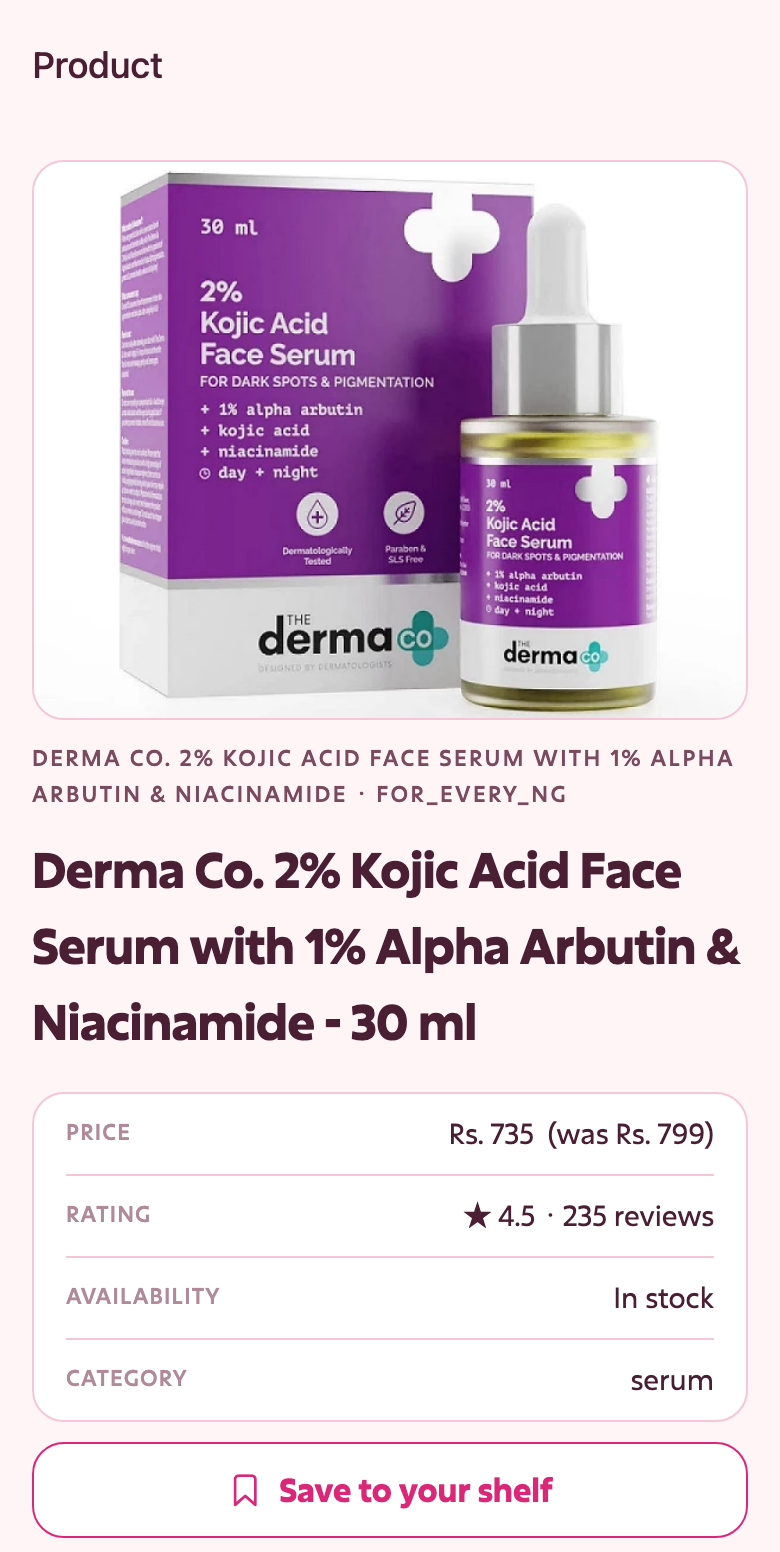
\includegraphics[width=\linewidth]{figures/product.png}\caption{Product detail}\end{subfigure}\\[8bp]
\begin{subfigure}[t]{0.24\linewidth}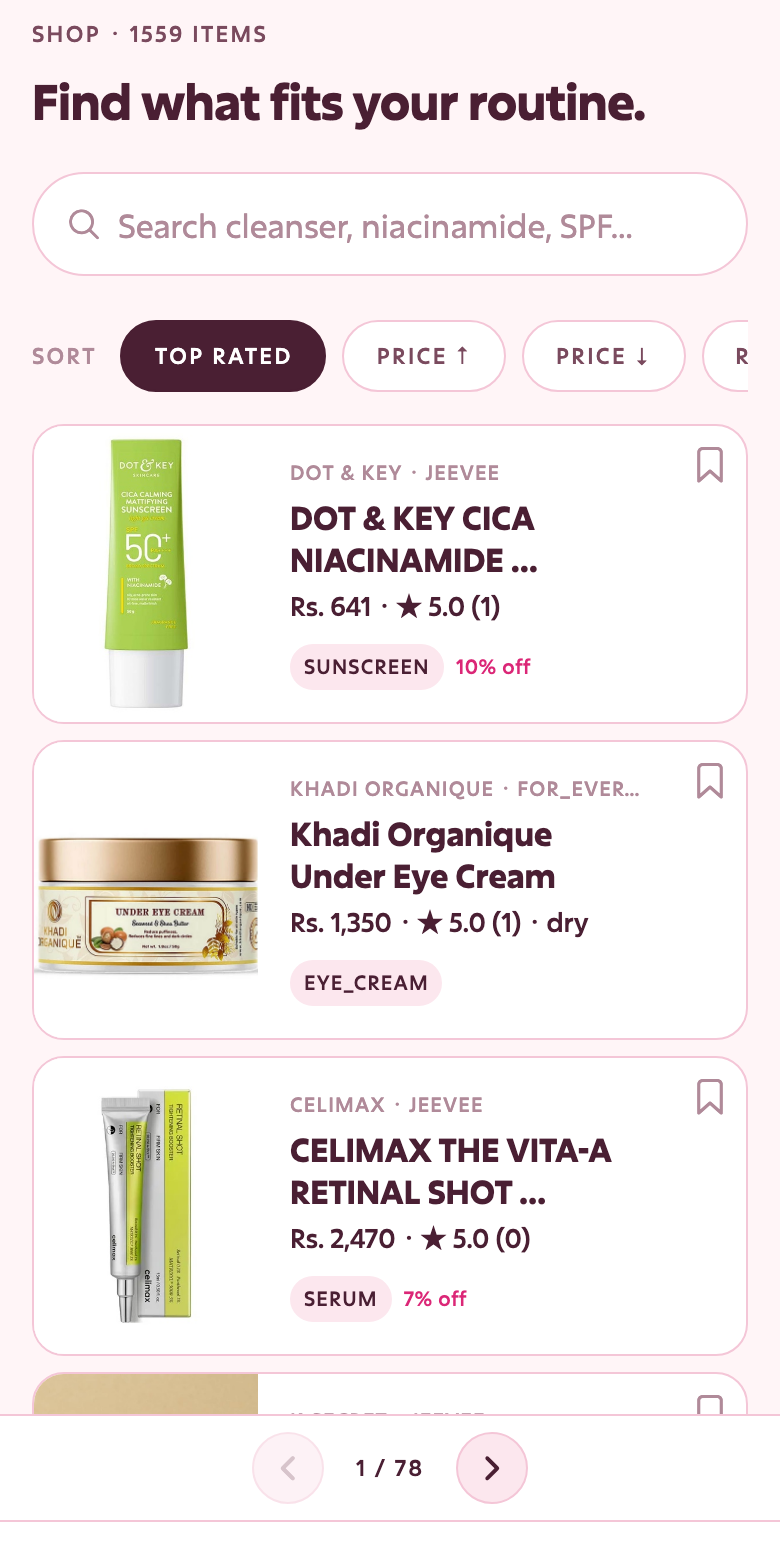
\includegraphics[width=\linewidth]{figures/catalog.png}\caption{Catalogue}\end{subfigure}\hfill
\begin{subfigure}[t]{0.24\linewidth}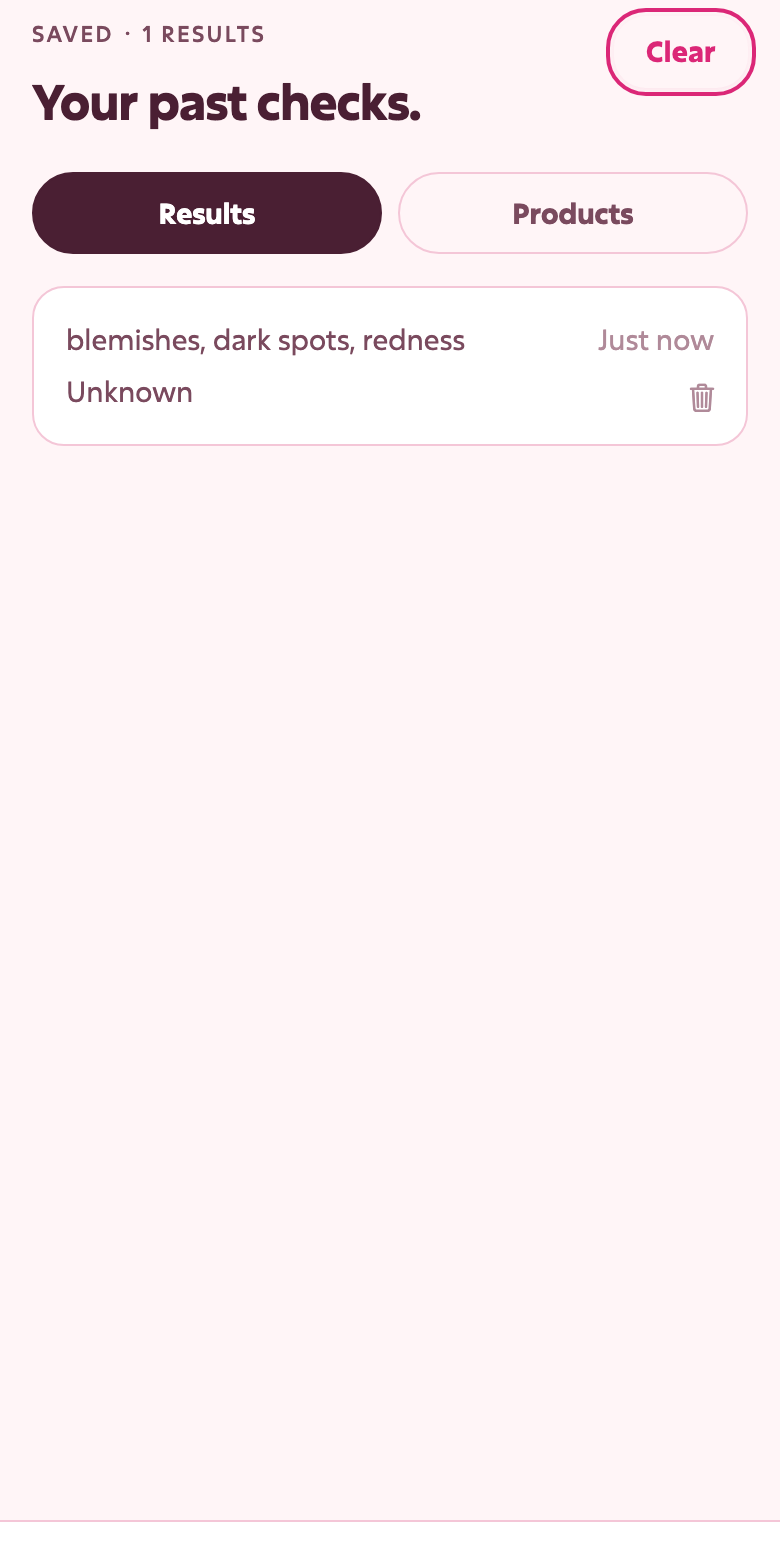
\includegraphics[width=\linewidth]{figures/history.png}\caption{History}\end{subfigure}\hfill
\begin{subfigure}[t]{0.24\linewidth}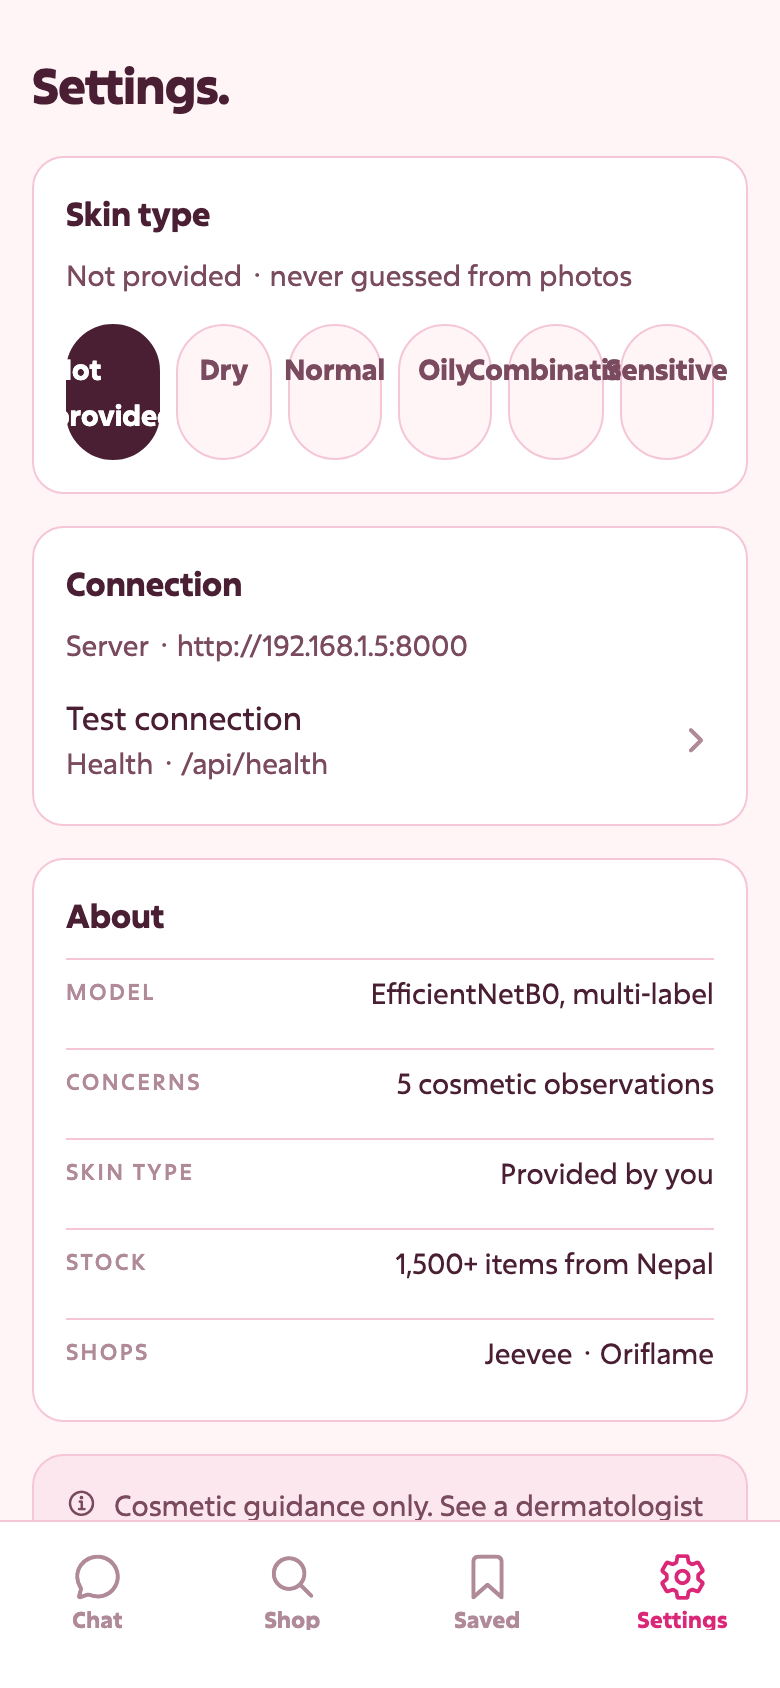
\includegraphics[width=\linewidth]{figures/settings.png}\caption{Settings}\end{subfigure}\hfill
\begin{subfigure}[t]{0.24\linewidth}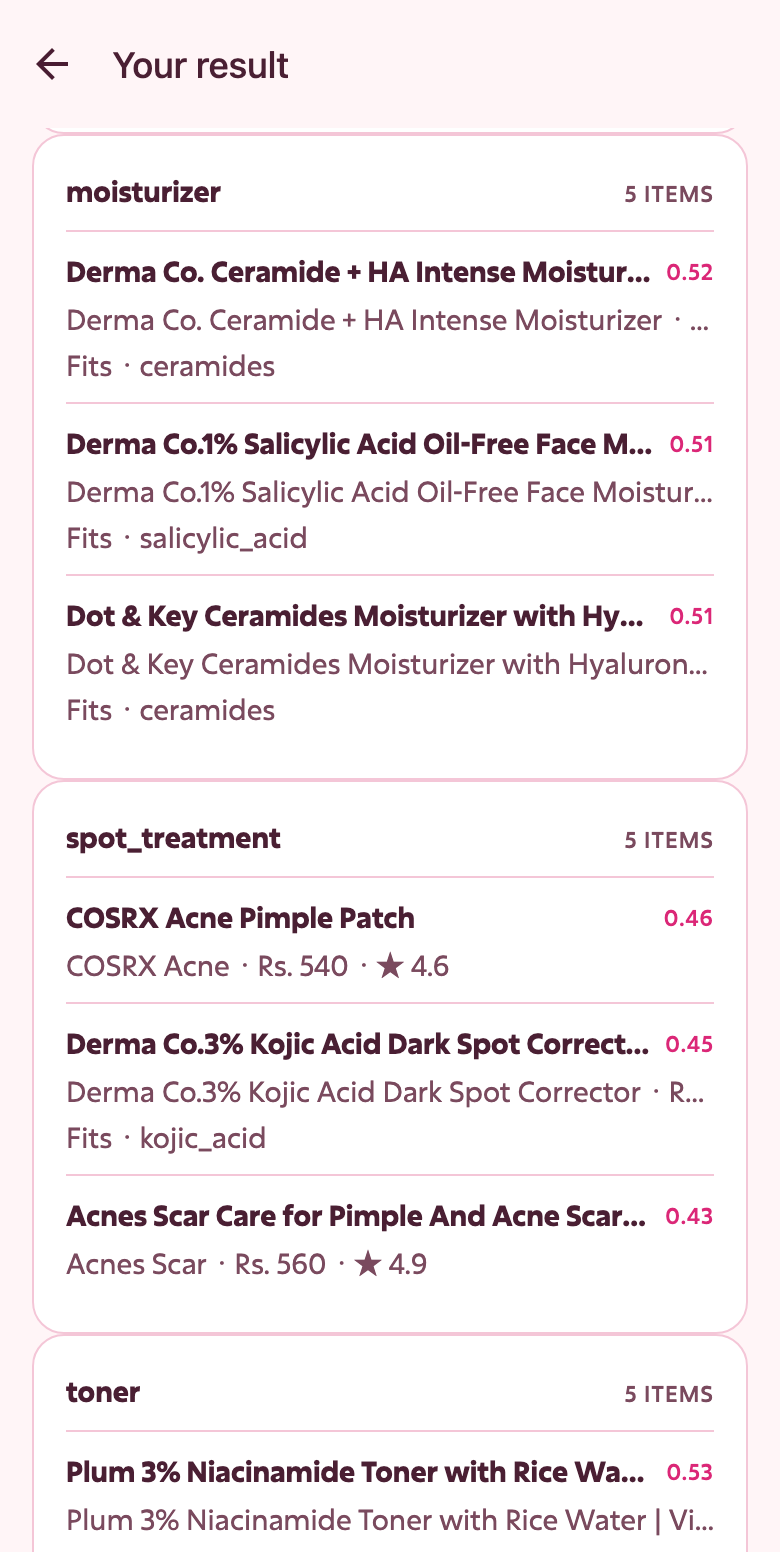
\includegraphics[width=\linewidth]{figures/analysis_2.png}\caption{More categories}\end{subfigure}
\caption{Screens from the running application (Expo web build, 390$\times$844 viewport). The analysed image is an FFHQ-Wrinkle test image.}
\label{fig:screens}
\end{figure}

\subsubsection*{Key development challenges}

Several practical problems consumed more time than planned. Each shaped the final design.

\begin{itemize}
  \item \textbf{Native photo upload.} On physical devices, photos selected in React Native could not be sent reliably as form data using the web-style \texttt{fetch} pattern. Uploads were rewritten to use \texttt{expo-file-system}. A 10\,MB size check was added on the client as well as the server, so that users receive an immediate, specific error rather than a generic failure.
  \item \textbf{Local networking.} The phone and the laptop running the backend must share a network, and the backend's address changes between networks. The client derives the server address from the Expo development host automatically. A ``Test connection'' diagnostic calls \texttt{/api/health} and reports exactly which URL failed. This turned a frequent source of confusion into a one-tap check.
  \item \textbf{Language-model integration.} Running Qwen2.5 inside the API process blocked other requests. Generation was moved to a worker thread behind an asynchronous lock. The analysis flow was made independent of the language model, and a rule-based fallback now answers when the model is slow, unavailable or returns invalid JSON.
  \item \textbf{Reproducibility.} After the preprocessing mismatch was discovered, a SHA-256 hash of the weights, the manifest paths and the preprocessing description were written into every evaluation file. This allows any reported number to be traced to the exact model and data that produced it.
\end{itemize}

These challenges map directly to the problem statement. Trustworthy guidance requires not only an accurate model, but also an application that fails clearly, explains its errors and can be reproduced.

\subsection{Validation and Testing}
\label{sec:validation}

Validation used five complementary kinds of evidence. All raw outputs are stored in \texttt{report/final/evidence/}.

\subsubsection*{Unit tests}

Nine test modules in \texttt{scripts/} were run. All passed, including a pipeline integration test that runs the real model and recommender end to end. Together they cover:
\begin{itemize}
  \item the API response contract;
  \item audit hashing;
  \item manifest and training logic (mask handling, balancing and non-overwrite);
  \item the SCIN quarantine;
  \item the language-model guardrail, which verifiably drops a fabricated product ID.
\end{itemize}
The suite is small, and only some of its checks are formal assertions.

\subsubsection*{Model performance on held-out data}

Table~\ref{tab:results} reports test metrics for the deployed \texttt{concern\_human\_reviewed} model. Thresholds were chosen on validation data. Figure~\ref{fig:results} compares F1, ROC-AUC and balanced accuracy, and Table~\ref{tab:modelcompare} compares all four model versions on the same test set.

\begin{table}[ht]
\centering\small
\caption{Held-out test performance of the deployed model (n = labelled test images per concern)}
\label{tab:results}
\setlength{\tabcolsep}{4pt}
\begin{tabular}{lrrrrrrrr}
\toprule
\textbf{Concern} & \textbf{n (+/--)} & \textbf{Thr.} & \textbf{Acc.} & \textbf{Prec.} & \textbf{Recall} & \textbf{F1} & \textbf{Bal.\,acc.} & \textbf{ROC-AUC}\\
\midrule
Blemishes & 101 (97/4) & 0.50 & 0.901 & 0.978 & 0.918 & 0.947 & 0.709 & 0.863\\
Dark spots & 87 (65/22) & 0.43 & 0.506 & 0.775 & 0.477 & 0.590 & 0.534 & 0.580\\
Redness & 105 (97/8) & 0.75 & 0.771 & 0.951 & 0.794 & 0.865 & 0.647 & 0.709\\
Visible pores & 55 (46/9) & 0.81 & 0.600 & 0.900 & 0.587 & 0.711 & 0.627 & 0.597\\
Fine lines & 234 (116/118) & 0.29 & 0.833 & 0.824 & 0.845 & 0.834 & 0.833 & 0.920\\
\midrule
\textbf{Macro} & 582 decisions & -- & 0.722 & 0.885 & 0.724 & \textbf{0.789} & \textbf{0.670} & \textbf{0.734}\\
\bottomrule
\end{tabular}

\vspace{2bp}{\footnotesize Pooled accuracy over all 582 known-label decisions: \textbf{76.3\%}. Macro PR-AUC: 0.904.}
\end{table}

\begin{figure}[ht]
\centering
\begin{tikzpicture}
\begin{axis}[
  ybar, bar width=9bp, width=0.92\linewidth, height=5.6cm,
  ymin=0, ymax=1.05, ylabel={Score}, ylabel style={font=\small},
  symbolic x coords={Blemishes,Dark spots,Redness,Visible pores,Fine lines},
  xtick=data, x tick label style={font=\small},
  yticklabel style={font=\small}, ymajorgrids, grid style={black!10},
  legend style={at={(0.5,1.03)},anchor=south,legend columns=3,font=\small,draw=none},
  enlarge x limits=0.14]
\addplot[fill=TemplateBlue!75,draw=none] coordinates {(Blemishes,0.947)(Dark spots,0.590)(Redness,0.865)(Visible pores,0.711)(Fine lines,0.834)};
\addplot[fill=Accent!70,draw=none] coordinates {(Blemishes,0.863)(Dark spots,0.580)(Redness,0.709)(Visible pores,0.597)(Fine lines,0.920)};
\addplot[fill=black!30,draw=none] coordinates {(Blemishes,0.709)(Dark spots,0.534)(Redness,0.647)(Visible pores,0.627)(Fine lines,0.833)};
\draw[dashed,black!60] (rel axis cs:0,0.476) -- (rel axis cs:1,0.476) node[pos=0.99,font=\scriptsize,anchor=south east,fill=white,inner sep=1bp]{chance = 0.5};
\legend{F1, ROC-AUC, Balanced accuracy}
\end{axis}
\end{tikzpicture}
\caption{F1 overstates performance when positives dominate; ROC-AUC and balanced accuracy show where the model discriminates}
\label{fig:results}
\end{figure}

\begin{table}[ht]
\centering\small
\caption{All model versions on the same held-out test set (582 known-label decisions)}
\label{tab:modelcompare}
\begin{tabularx}{\linewidth}{P{3.6cm}rrrrY}
\toprule
\textbf{Model} & \textbf{Pooled acc.} & \textbf{Macro F1} & \textbf{Bal.\,acc.} & \textbf{ROC-AUC} & \textbf{Decision}\\
\midrule
\texttt{concern\_v2} (first labels) & 73.2\% & 0.779 & 0.635 & 0.717 & Replaced\\
Class-balanced candidate & 74.6\% & 0.736 & 0.617 & 0.708 & Rejected: redness specificity 0\\
\textbf{Human-reviewed (deployed)} & \textbf{76.3\%} & \textbf{0.789} & \textbf{0.670} & 0.734 & \textbf{Deployed}\\
Human-reviewed + MEMI melasma & 69.8\% & 0.701 & 0.662 & 0.750 & Rejected: accuracy fell\\
\bottomrule
\end{tabularx}
\end{table}

Three results stand out.
\begin{itemize}
  \item \textbf{Fine lines are learned well.} On the only balanced concern, the model reaches an ROC-AUC of 0.920 and a balanced accuracy of 0.833, up from 0.911 and 0.795.
  \item \textbf{More negative labels helped where they were added.} Redness accuracy rose from 55.2\% to 77.1\%, although its balanced accuracy barely changed (0.643 to 0.647). Blemish balanced accuracy rose from 0.610 to 0.709, and pores from 0.560 to 0.627. Even so, the test set still holds only 4 negative blemish images and 8 negative redness images, so these figures move by large steps when a single image changes. The high F1 scores for blemishes and redness still flatter the model: with 97 positives and 4 negatives, always saying ``present'' would give F1 $\approx$ 0.98.
  \item \textbf{Dark spots did not improve.} Dark-spot accuracy fell from 64.4\% to 50.6\% and ROC-AUC stayed at about 0.58. The deployed model is the best overall, but it is worse than \texttt{concern\_v2} on this one concern, and dark-spot output should be treated as unreliable.
\end{itemize}

\textbf{Run-to-run variation.} Training on the Apple GPU (tensorflow-metal) was not fully reproducible: retraining the same recipe with the same seed gave 72.2\% and 78.9\% macro accuracy. Over three runs, the human-reviewed recipe averaged 74.4\% macro accuracy and 0.746 ROC-AUC. Differences of a few points between single runs are therefore within noise. The deployed weights are the stored run whose metrics are reported above, identified by the SHA-256 hash in its evaluation file.

\textbf{Learning curve.} To test whether more data would help, the model was retrained on 25, 50, 75 and 100\% of the earlier gold training set (150 to 600+ images), with two seeds each (Figure~\ref{fig:lc}). ROC-AUC rose with data for blemishes (0.53 to 0.71) and pores (0.45 to 0.68). Dark spots stayed near 0.55. Fine lines were already at about 0.97 on that smaller, easier test set.

These trends suggest that more labelled data would help most concerns, but that dark spots may also need a better label definition. The run-to-run standard deviation (up to 0.20 for blemishes) is large relative to the gains, so these trends are indicative only.

\begin{figure}[ht]
\centering
\begin{tikzpicture}
\begin{axis}[width=0.82\linewidth,height=5.4cm,xlabel={Training images},ylabel={Test ROC-AUC},
  xtick={159,318,477,636},ymin=0.4,ymax=1.02,ymajorgrids,grid style={black!10},
  legend style={font=\scriptsize,at={(1.02,0.5)},anchor=west,draw=none},
  label style={font=\small},tick label style={font=\small}]
\addplot[mark=*,TemplateBlue,thick] coordinates {(159,0.530)(318,0.593)(477,0.756)(636,0.706)};
\addplot[mark=square*,Accent,thick] coordinates {(159,0.511)(318,0.530)(477,0.547)(636,0.547)};
\addplot[mark=triangle*,orange!80!black,thick] coordinates {(159,0.593)(318,0.703)(477,0.691)(636,0.694)};
\addplot[mark=diamond*,teal,thick] coordinates {(159,0.454)(318,0.579)(477,0.575)(636,0.682)};
\addplot[mark=o,black!60,thick] coordinates {(159,0.967)(318,0.984)(477,0.986)(636,0.981)};
\legend{Blemishes,Dark spots,Redness,Pores,Fine lines}
\end{axis}
\end{tikzpicture}
\caption{Learning curve (mean of two seeds, earlier gold manifests)}
\label{fig:lc}
\end{figure}

\textbf{Negative experiments.} Two candidates were rejected (Table~\ref{tab:modelcompare}). Class reweighting slightly improved validation ROC-AUC (0.686 to 0.698), but on the test set macro F1 fell to 0.736 and redness specificity dropped to 0, with all eight negatives misclassified. Adding MEMI melasma photos raised macro ROC-AUC to 0.750 but lowered pooled accuracy to 69.8\% and left dark-spot ROC-AUC near chance (0.57). Both results point the same way: reweighting or adding positives cannot create the variety of \emph{negative} examples that is missing from the data.

\subsubsection*{Face-gate validation}

The YuNet gate (threshold 0.9) rejected all 300 PASCAL VOC non-face images. It was then run on every held-out test image to check how it would treat real inputs (Table~\ref{tab:gate}).

\begin{table}[ht]
\centering\small
\caption{Face-gate pass rate on held-out test images}
\label{tab:gate}
\begin{tabular}{lrrr}
\toprule
\textbf{Source / framing} & \textbf{Images} & \textbf{Passed} & \textbf{Rate}\\
\midrule
FFHQ-Wrinkle, full face & 211 & 211 & 100\%\\
Kaggle concerns, full face & 40 & 34 & 85\%\\
Original conditions, full face & 23 & 19 & 83\%\\
ACNE04, full face & 15 & 11 & 73\%\\
Kaggle concerns, close-up & 106 & 64 & 60\%\\
Original conditions, close-up & 54 & 14 & 26\%\\
ACNE04, close-up & 30 & 20 & 67\%\\
\midrule
\textbf{All} & 479 & 373 & \textbf{77.9\%}\\
\bottomrule
\end{tabular}
\end{table}

Of the held-out images, 22\% would be rejected by the deployed app before reaching the model. Most were facial close-ups, the framing that carries most of the blemish, pore and dark-spot labels. The model metrics therefore describe a wider input range than the app accepts. Conversely, the app never sees many of the close-ups on which the concern model was trained. This mismatch between the gate and the model is discussed in Section~\ref{sec:eval}.

\subsubsection*{Functional testing}

Nineteen black-box test cases were executed against the running API with \texttt{curl}. They were first run on 30 September 2026 and re-run on 1 October 2026 after the human-reviewed model was deployed. Appendix~\ref{app:tests} lists them in full, and Table~\ref{tab:funcsummary} summarises the re-run. Eighteen passed. One failed: TC15, the chat question. In the first run it returned a grounded reply after 55\,s. In the re-run it gave no response within 240\,s, and a retry also timed out after 500\,s. The cause is a design weakness: chat generations run one at a time behind a lock with no timeout, so a request that the client has abandoned keeps running and blocks every later one. Warm analysis latency over 10 runs had a median of 0.18\,s (maximum 0.24\,s) on an Apple M4 CPU, which satisfies N4.

\begin{table}[ht]
\centering\small
\caption{Functional test summary (details in Appendix~\ref{app:tests})}
\label{tab:funcsummary}
\begin{tabularx}{\linewidth}{lrrY}
\toprule
\textbf{Area} & \textbf{Cases} & \textbf{Pass} & \textbf{Observation}\\
\midrule
Analysis, valid input & 5 & 5 & Skin type correctly changes ranking (TC18/19); a false face rejection occurred in the first run (TC02)\\
Health \& input validation & 6 & 6 & Correct 400/422 codes; the corrupt-image message exposes an internal Python object name\\
Products \& metadata & 6 & 6 & Search, filter, 404 and categories correct\\
Chat & 2 & 1 & Empty message rejected; question answered in 55\,s in the first run but timed out in the re-run (TC15)\\
\midrule
\textbf{Total} & 19 & 18 & \\
\bottomrule
\end{tabularx}
\end{table}

\subsubsection*{Usability: heuristic evaluation}

The running application was first inspected against Nielsen's ten heuristics \citep{galavi2024}. The inspection used the screens in Figure~\ref{fig:screens} and a cognitive walkthrough of the ``check a photo, then read recommendations'' task. Severity was rated from 0 (not a problem) to 4 (catastrophe). Because the evaluator also built the system, problems may be missed or rated leniently, so these findings are complemented by the participant survey below.

\begin{table}[ht]
\centering\small
\caption{Heuristic evaluation findings (author-conducted; severity 0--4)}
\label{tab:heuristic}
\begin{tabularx}{\linewidth}{P{3.3cm}Yc}
\toprule
\textbf{Heuristic} & \textbf{Finding} & \textbf{Sev.}\\
\midrule
Match with real world & The evening routine lists ``broad-spectrum sunscreen'' because the routine is split into morning and evening by position, not by step type & 3\\
Aesthetic \& minimalist & Chat replies show raw Markdown (\texttt{**bold**}) instead of formatted text & 2\\
Consistency \& standards & Settings chips truncate labels (``Not provided'' is clipped; ``Combination'' and ``Sensitive'' overlap) on a 390\,px screen & 2\\
Consistency \& standards & The About panel lists ``Jeevee $\cdot$ Oriflame'' but omits ForEveryNG, which supplies 41\% of products & 1\\
Error prevention & Close-up photos are rejected with ``No face found'' although the concern model can analyse them & 3\\
Visibility of system status & Chat gives no progress indication during a response that can take about 55\,s on CPU & 2\\
Help users with errors & Rejections give an actionable retake instruction; network errors are translated into plain language & 0\\
Recognition vs.\ recall & Score bars show a threshold tick and a status label, so users need not remember what a score means & 0\\
Accuracy of content & Some products sit in the wrong category (a body wash appears under ``toner'') because of keyword categorisation & 2\\
Code quality (dev) & React warning: \texttt{<button>} nested in \texttt{<button>} on the history and result screens (invalid markup; accessibility risk) & 1\\
\bottomrule
\end{tabularx}
\end{table}

\subsubsection*{Usability: participant survey}
\label{sec:survey}

Participants used the app on their own phones and then completed an anonymous Google Form (protocol and questions in Appendix~\ref{app:usability}). Each participant carried out four tasks: check a face photo, read and interpret the result, find and save a recommended product, and ask the assistant a question. For each task they reported whether they completed it and rated its ease from 1 (very difficult) to 5 (very easy). They then completed the ten-item System Usability Scale (SUS), scored from 0 to 100, where about 68 is the usual benchmark for average usability \citep{vlachogianni2022}. Finally, they answered questions on whether they understood the ``uncertain'' label, noticed the disclaimer, and would trust or buy the recommended products. Responses were exported from Google Forms as CSV and analysed with a script stored in \texttt{evidence/user\_study/}.

% TODO(user): fill from the exported responses CSV -- run
%   python3 evidence/user_study/analyse_sus.py responses.csv
% and paste the real figures below. Do not invent values.
\begin{table}[ht]
\centering\small
\caption{Participant survey results (n = [TODO])}
\label{tab:survey}
\begin{tabularx}{\linewidth}{lY}
\toprule
\textbf{Measure} & \textbf{Result}\\
\midrule
Participants & [TODO: n, age bands, skin types]\\
Task 1: check a photo & [TODO: completion \%, mean ease]\\
Task 2: read the result & [TODO]\\
Task 3: find and save a product & [TODO]\\
Task 4: ask the assistant & [TODO]\\
SUS score & [TODO: mean (SD), range]\\
Understood ``uncertain'' & [TODO: \% yes]\\
Noticed disclaimer & [TODO: \% yes]\\
Would trust / buy recommendations & [TODO: mean 1--5]\\
\bottomrule
\end{tabularx}
\end{table}

[TODO: two or three sentences summarising the main themes from the open comments, quoting participants only with their permission.]

